\documentclass[tikz,border=15pt]{standalone}
\usepackage{amsmath, amssymb}
\usetikzlibrary{matrix, positioning, arrows.meta, fit, shapes.geometric, calc, backgrounds}

\begin{document}
	
	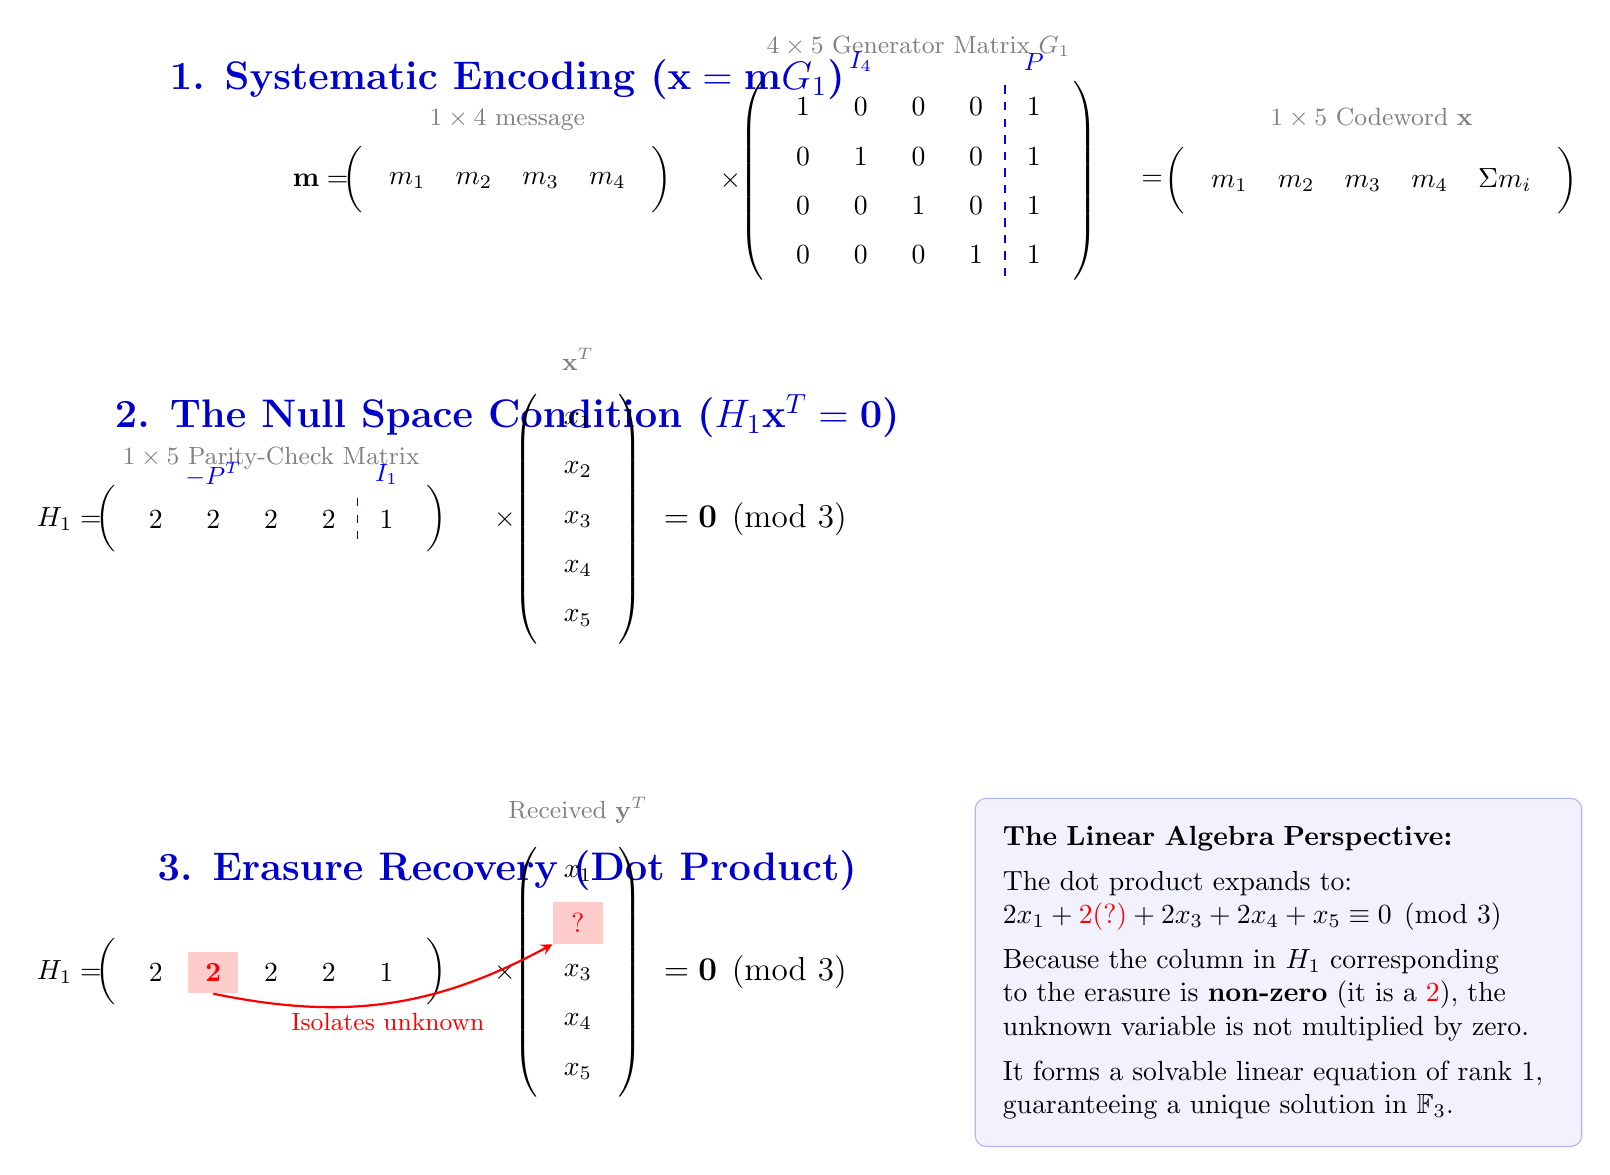
\begin{tikzpicture}[
		>=stealth,
		% FIXED: Removed align=center from nodes={...} so math mode isn't broken
		mymatrix/.style={matrix of math nodes, left delimiter=(, right delimiter=), inner sep=4pt, row sep=0.1cm, column sep=0.1cm, nodes={minimum width=1.8em, minimum height=1.5em}},
		explain/.style={text width=7cm, align=left, font=\normalsize, fill=blue!5, rounded corners, inner sep=10pt, draw=blue!30},
		title/.style={font=\Large\bfseries, text=blue!80!black}
		]
		
		% ==========================================
		% 1. ENCODING: m * G = x
		% ==========================================
		\node[title] (enc_title) {1. Systematic Encoding ($\mathbf{x} = \mathbf{m}G_1$)};
		
		\matrix[mymatrix, below=0.5cm of enc_title] (m) {
			m_1 & m_2 & m_3 & m_4 \\
		};
		\node[left=0.1cm of m] {$\mathbf{m} = $};
		\node[above=0.1cm of m, font=\small, text=gray] {$1 \times 4$ message};
		
		\matrix[mymatrix, right=1.5cm of m] (G) {
			1 & 0 & 0 & 0 & 1 \\
			0 & 1 & 0 & 0 & 1 \\
			0 & 0 & 1 & 0 & 1 \\
			0 & 0 & 0 & 1 & 1 \\
		};
		\node[left=0.2cm of G] {$\times$};
		\node[above=0.1cm of G, font=\small, text=gray] {$4 \times 5$ Generator Matrix $G_1$};
		
		% Draw block matrix dividers for G
		\draw[dashed, blue] ($(G-1-4.north east)!0.5!(G-1-5.north west)$) -- ($(G-4-4.south east)!0.5!(G-4-5.south west)$);
		\node[blue, font=\small] at ($(G-1-2.north)+(0,0.3)$) {$I_4$};
		\node[blue, font=\small] at ($(G-1-5.north)+(0,0.3)$) {$P$};
		
		\matrix[mymatrix, right=1.5cm of G] (x) {
			m_1 & m_2 & m_3 & m_4 & \Sigma m_i \\
		};
		\node[left=0.2cm of x] {$=$};
		\node[above=0.1cm of x, font=\small, text=gray] {$1 \times 5$ Codeword $\mathbf{x}$};
		
		% ==========================================
		% 2. NULL SPACE / PARITY CHECK
		% ==========================================
		\node[title, below=3.5cm of enc_title] (chk_title) {2. The Null Space Condition ($H_1 \mathbf{x}^T = \mathbf{0}$)};
		
		\matrix[mymatrix, below=0.5cm of chk_title, xshift=-3cm] (H) {
			2 & 2 & 2 & 2 & 1 \\
		};
		\node[left=0.1cm of H] {$H_1 = $};
		\node[above=0.1cm of H, font=\small, text=gray] {$1 \times 5$ Parity-Check Matrix};
		
		% Draw block matrix dividers for H
		\draw[dashed, blue] ($(H-1-4.north east)!0.5!(H-1-5.north west)$) -- ($(H-1-4.south east)!0.5!(H-1-5.south west)$);
		\node[blue, font=\small] at ($(H-1-2.north)+(0,0.3)$) {$-P^T$};
		\node[blue, font=\small] at ($(H-1-5.north)+(0,0.3)$) {$I_1$};
		
		\matrix[mymatrix, right=1.5cm of H] (xT) {
			x_1 \\ x_2 \\ x_3 \\ x_4 \\ x_5 \\
		};
		\node[left=0.2cm of xT] {$\times$};
		\node[above=0.1cm of xT, font=\small, text=gray] {$\mathbf{x}^T$};
		
		\node[right=0.5cm of xT, font=\large] (zero) {$= \mathbf{0} \pmod 3$};
		
		% ==========================================
		% 3. ERASURE AS A LINEAR SYSTEM
		% ==========================================
		\node[title, below=5cm of chk_title] (rec_title) {3. Erasure Recovery (Dot Product)};
		
		\matrix[mymatrix, below=0.5cm of rec_title, xshift=-3cm] (H2) {
			2 & |[fill=red!20, text=red]| \mathbf{2} & 2 & 2 & 1 \\
		};
		\node[left=0.1cm of H2] {$H_1 = $};
		
		\matrix[mymatrix, right=1.5cm of H2] (yT) {
			x_1 \\ |[fill=red!20, text=red]| \mathbf{?} \\ x_3 \\ x_4 \\ x_5 \\
		};
		\node[left=0.2cm of yT] {$\times$};
		\node[above=0.1cm of yT, font=\small, text=gray] {Received $\mathbf{y}^T$};
		
		\node[right=0.5cm of yT, font=\large] (zero2) {$= \mathbf{0} \pmod 3$};
		
		% Connection arrows to show the dot product targeting the unknown
		\draw[->, red, thick, bend right=20] (H2-1-2.south) to node[below, font=\small] {Isolates unknown} (yT-2-1.south west);
		
		\node[explain, right=1.5cm of zero2] (eq) {
			\textbf{The Linear Algebra Perspective:}\\[1ex]
			The dot product expands to:\\
			$2x_1 + \color{red}2(?)\color{black} + 2x_3 + 2x_4 + x_5 \equiv 0 \pmod 3$\\[1ex]
			Because the column in $H_1$ corresponding to the erasure is \textbf{non-zero} (it is a $\color{red}2$), the unknown variable is not multiplied by zero. \\[1ex]
			It forms a solvable linear equation of rank 1, guaranteeing a unique solution in $\mathbb{F}_3$.
		};
		
	\end{tikzpicture}
	
\end{document}